\chapter{System Geometry}
\subsection{Ball's translational position and velocity}
In oder to get the system's variable right , we need to analyze the system geometry correctly.
In the \figref{SystemGeometry} we can see that the ball's center is positioned according to the distance $p$ and angle $\theta$.
But in order to find the ball's position in Cartesian , we need to transform the ball's position in terms of $x(p,\theta)$ and $y(p,\theta)$.
This will help us later when we need to change some variables from and to polar coordinates.
That we can achieve with calculating the distance from the center of rotation to the center of the ball. 

\begin{figure}[h]
	\centering
	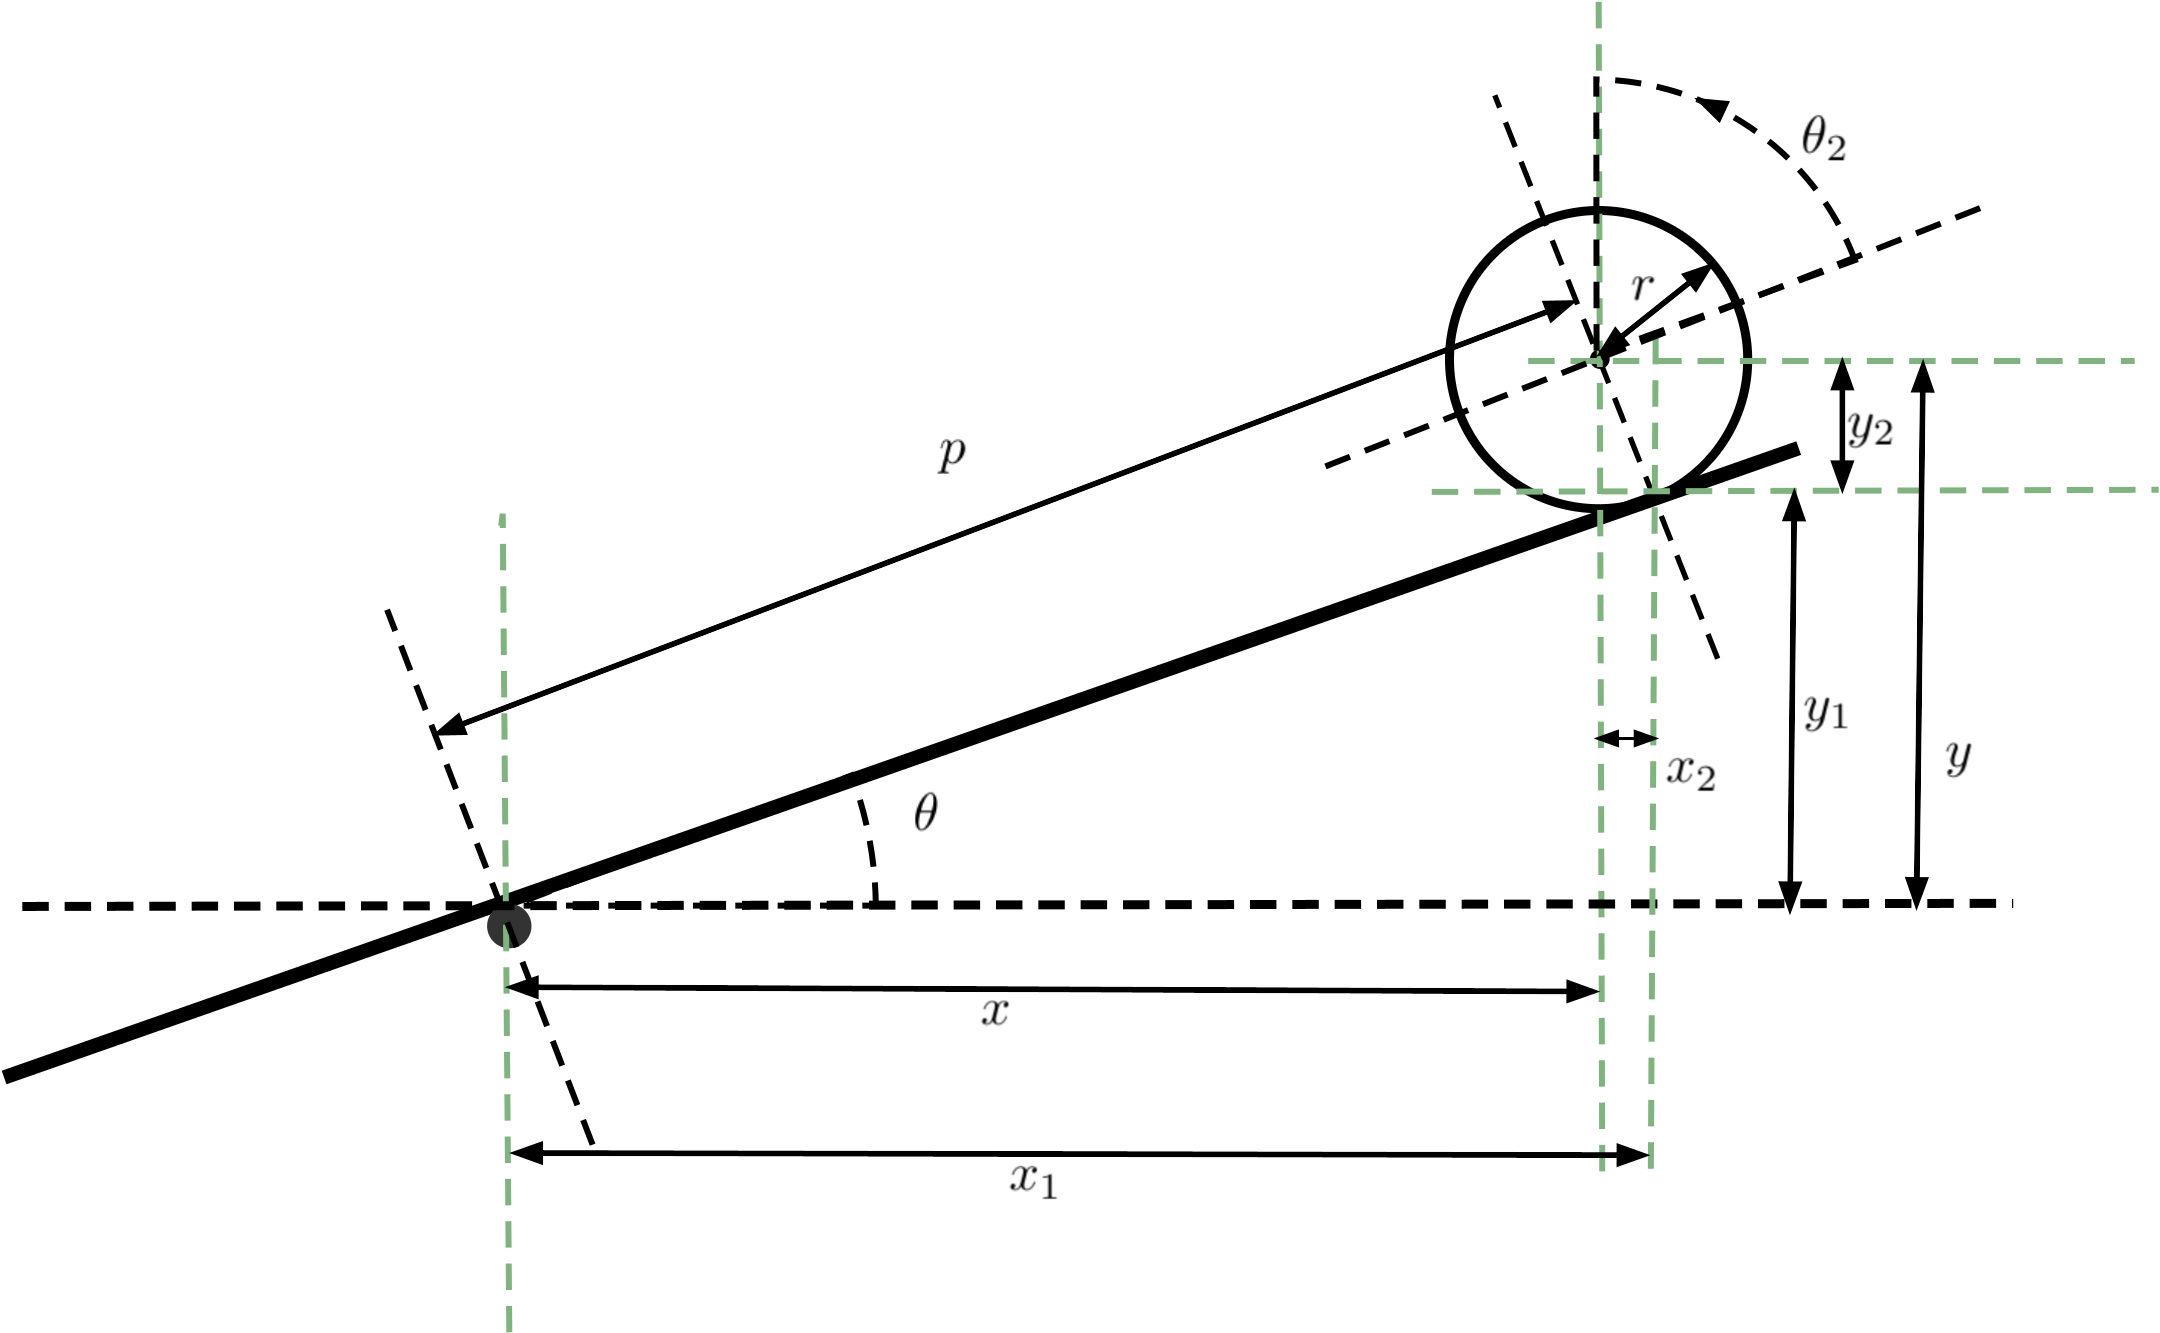
\includegraphics[height =7.5cm,width =10cm]{System_Geo}
	\caption{System Geometry}\label{SystemGeometry}
\end{figure}
\newpage
First we will consider the following while observing the \figref{SystemGeometry}:
\begin{equation}
	\begin{split}
		x = x_1 - x_2 \\
		y = y_1 + y_2 
	\end{split}
\end{equation}
Now using some trigonometry with the triangles in \figref{SystemGeometry_Triangles} we can get the following:
\begin{equation}
	\begin{split}
		x_1 = p.\cos{\theta} \\
		x_2 = r.\sin{\theta} \\
		y_1 = p.\sin{\theta} \\
		y_2 = r.\cos{\theta} 
	\end{split}
\end{equation}

\begin{figure}[h]
	\centering
	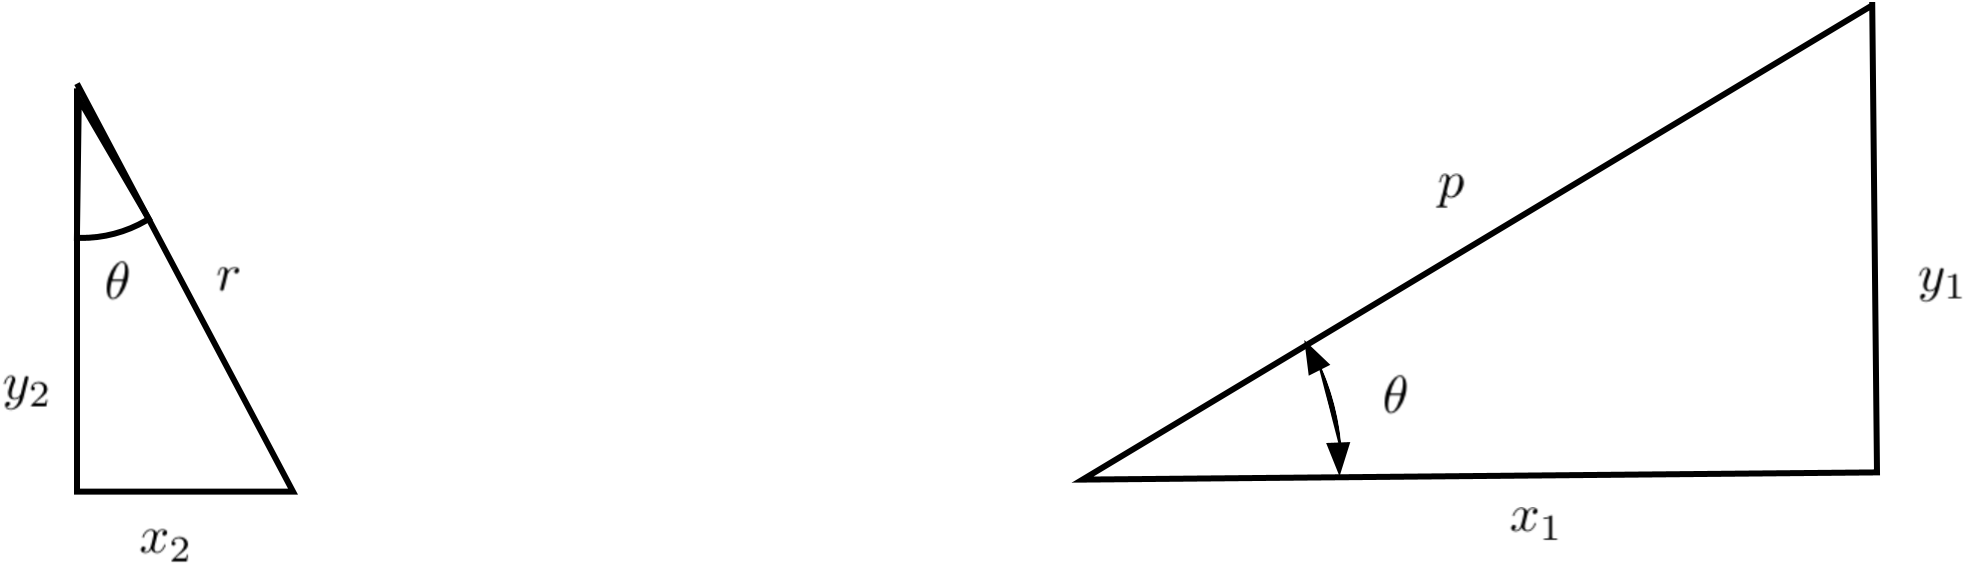
\includegraphics[height =4cm,width =8cm]{Triangles_System_Geo}
	\caption{Position Triangles}\label{SystemGeometry_Triangles}
\end{figure}
Lastly we substitute the values from (2) in (1):
\begin{equation}
	\begin{split}
		x = p.\cos{\theta} - r.\sin{\theta}\\
		y = p.\sin{\theta} + r.\cos{\theta}
	\end{split}
\end{equation}
It is also would be helpful , to calculate the velocity of the ball by taking the derivative of the position in respect to time.

\begin{equation}
	\begin{split}
		\dot{x}  = \dot{p}.\cos{\theta}-p.\theta'.\sin{\theta} - r.\theta'.\sin{\theta} \\
		\dot{y}  = \dot{p}.\sin{\theta}+ p.\theta'\cos{\theta} - r.\theta'.\sin{\theta} 
	\end{split}
\end{equation}
\newpage
\subsection{Ball's rotational position and velocity}
Now we need to find a relationship between the ball's angular values and the system variables $p$ and $\theta$.
By looking at the \figref{Angles_System_Geo} , we can tell that before tilting the system , the coordinates are normal and vertical.
After tilting the system and before the ball starts to roll , the coordinates are tilted by the amount of $\theta$,and the the ball starts to roll down, where 
a displacement of the angle is created $\alpha$,which is called the angular position of the ball.
This creates a new angle called (total displacement of the ball after tilting)$\sigma$ which is simply the sum of the two angles , and it's also equal to the position over the radius.

\begin{figure}[h]
	\centering
	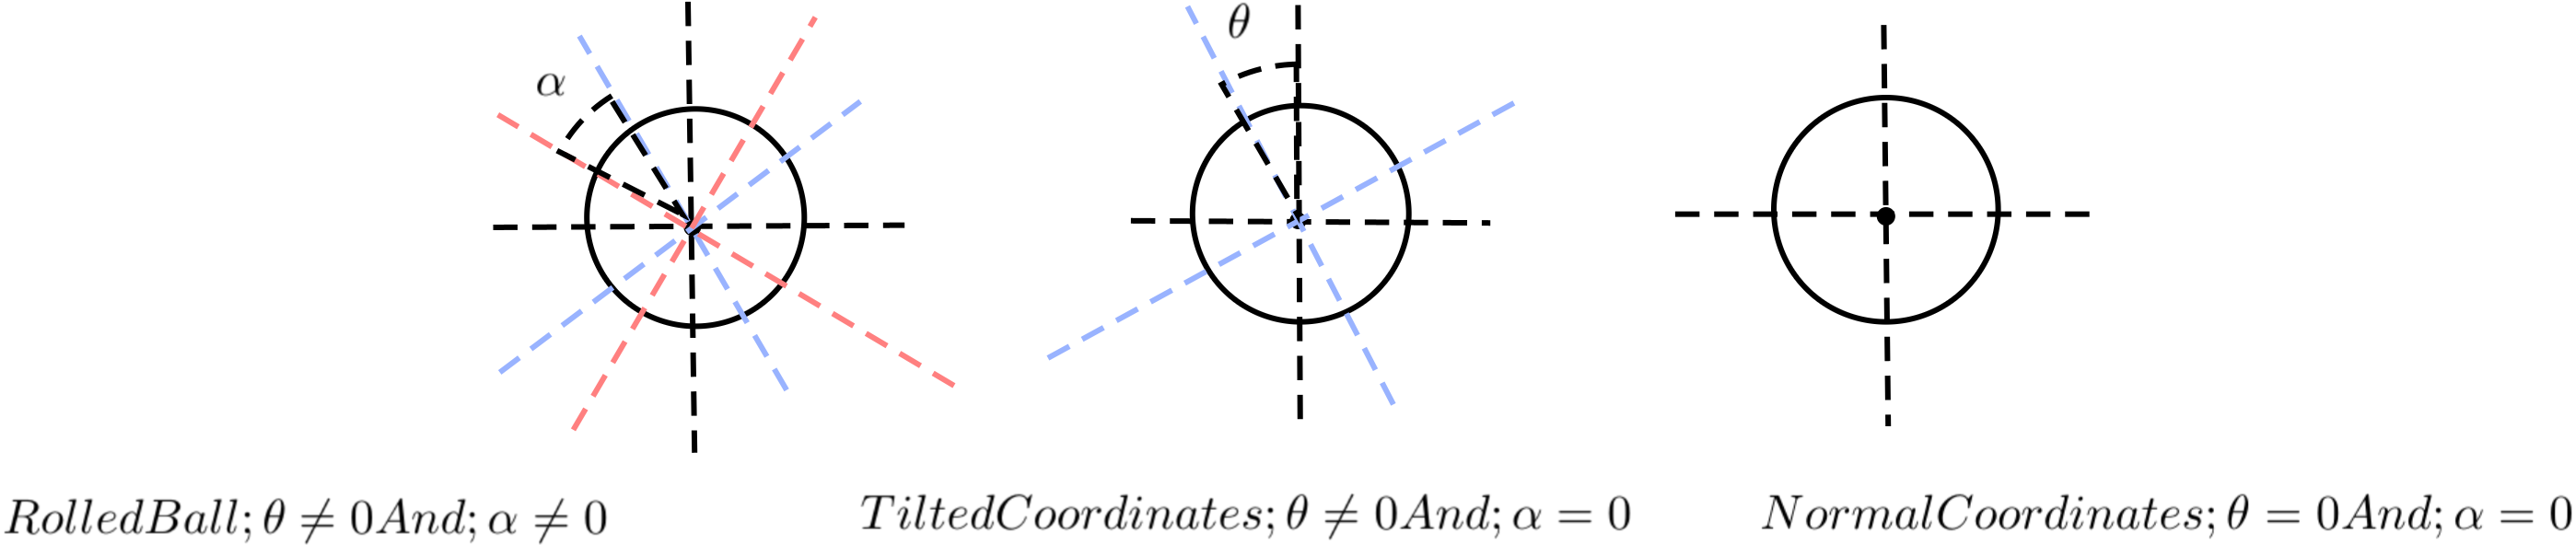
\includegraphics[height = 4cm,width =12cm]{Angles_System_Geo}
	\caption{Angular position}\label{Angles_System_Geo}
\end{figure}
Now to calculate $\alpha$:
\begin{equation}
	\begin{split}
		\sigma = \alpha + \theta \\
		\alpha = \theta - \sigma \\
		\alpha = \theta - \dfrac{p}{r}		
	\end{split}
\end{equation}
Now simply by taking the derivative of that we can calculate the angular velocity:
\begin{equation}
	\begin{split}
		\omega = \dot{\alpha} = \dot{\theta} - \dfrac{\dot{p}}{r}
	\end{split}
\end{equation}

Also the Moment of inertia of the ball is : 
\begin{equation}
	\begin{split}
		I_{\text{ball}} = \dfrac{2}{5}.m_{\text{ball}}.r^2
	\end{split}
\end{equation}
\newpage
\subsection{Beam Geometry}
The most important thing is to consider that the beam height is a changeable variable according to $\theta$.
The beam height sets in a relation to the total potential energy of the system which will be needed to get the system model.
Normally the beam \figref{Beam_System_Geo} sets at a height of $h$ ,but when tilted , it changes according to the $\cos{\theta}$.
Therefore:
\begin{equation}
	\begin{split}
		h = N.\cos{\theta}
	\end{split}
\end{equation}
\begin{figure}[h]
	\centering
	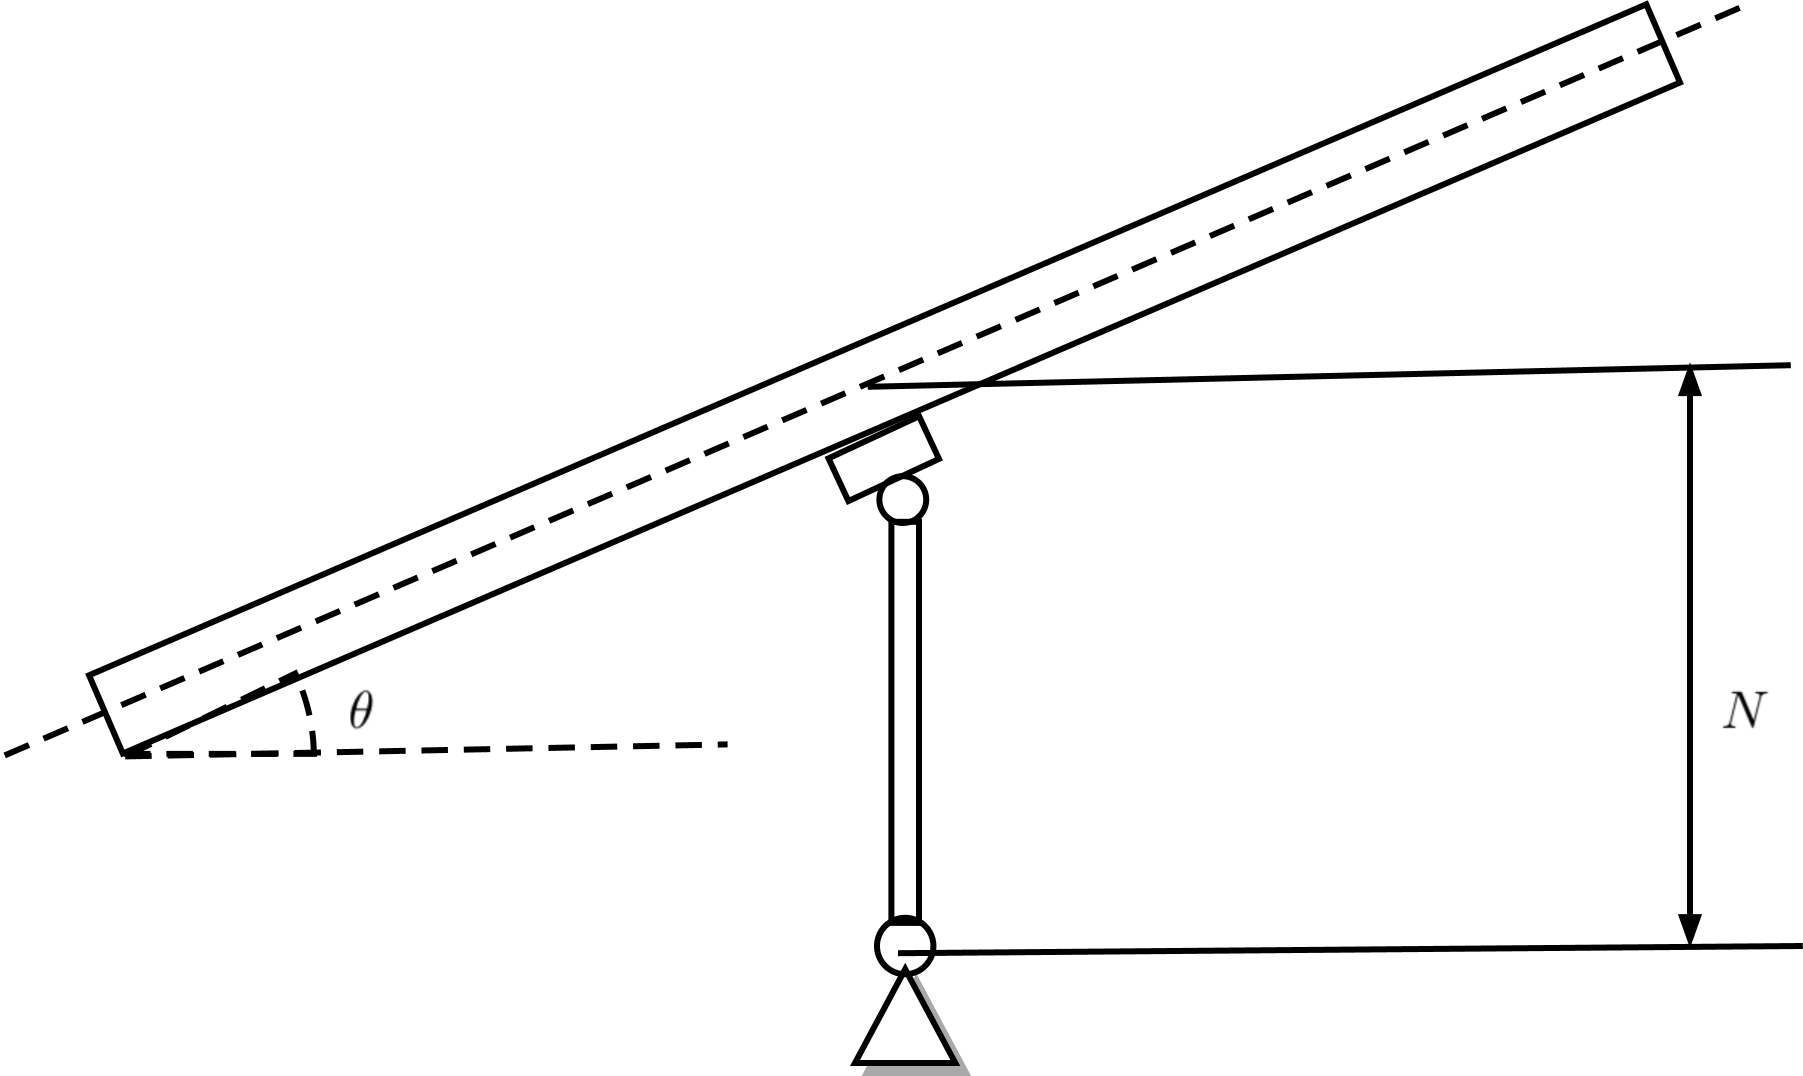
\includegraphics[height = 4cm,width =8cm]{Beam_System_Geo}
	\caption{Beam geometry}\label{Beam_System_Geo}
\end{figure}

\noindent Finally its important to say ,that there are more geometry to be done on the system , but for the peropus of this study we will ignore them in order to simplify the system.